\documentclass[compress, notes=hide]{beamer}
%\documentclass[compress, notes=hide,handout]{beamer}

\usepackage[english,norsk]{babel} %norske navn rundt omkring
\usepackage{lmodern}
\usepackage[T1]{fontenc} %Norsk tegnsetting (���)
\usepackage[latin1]{inputenc} %Norsk tegnsetting
\usepackage{amsmath,amsfonts,amssymb,mathrsfs} %matematikksymboler
\usepackage{algorithm, algorithmic}
\usepackage{amsthm} %for � lage teoremer og lignende.
\usepackage{bm} %fikser bold math-problematikken
%\usepackage[hang]{subfigure} %hvis du vil kunne ha flere figurer inni en figur
%\usepackage[small,bf,hang]{caption} %bestemmer format p� figurtekst
\usepackage{multirow}
\usepackage{graphpap}
\usepackage{pgf} %Tegning
\def\pgfex{ex}
%\usepackage{mathptmx}
%\usepackage{helvet}
%\usepackage{verbatim}

\setbeamertemplate{caption}[]
\setbeamertemplate{navigation symbols}{}
%\setbeamertemplate{footline}[page number]
\setbeamertemplate{footline}[frame number]
%\setbeamertemplate{caption}[numbered] 
\usecolortheme{default}
%\usetheme{Pittsburgh} %\usetheme{Singapore}
\setbeamertemplate{itemize item}[circle] %triangel p� 2-level-itemize (for 1-level brukt {itemize item})
\setbeamertemplate{itemize subitem}[triangle] %triangel p� 2-level-itemize (for 1-level brukt {itemize item})
\setbeamertemplate{section in toc}[circle]{} %Nummer i table of content
\setbeamertemplate{enumerate items}[circle] 
\setbeamertemplate{itemize subitem}[triangle] %triangel p� 2-level-itemize (for 1-level brukt {itemize item})
\setbeamercolor{itemize subitem}{fg=gray} %farge bullets

% For � skrive i default bl� farge:
% \textcolor[rgb]{0.2,0.2,0.7}{Blablabla-tekst}
%\newcommand{\hl}[1]{\textcolor[rgb]{0.2,0.2,0.7}{\emph{#1}}}
\newcommand{\hl}[1]{\textbf{#1}}
\newcommand{\hlb}[1]{\textcolor[rgb]{0.2,0.2,0.7}{#1}}
\newcommand{\sectionheader}{
    \usebeamerfont*{section number projected}%
    \usebeamercolor{section number projected}%
    \begin{pgfpicture}{-1ex}{-0.4ex}{1ex}{2ex}
      \color{bg}
      \pgfpathcircle{\pgfpoint{0pt}{.75ex}}{1.2ex}
      \pgfusepath{fill}
      \pgftext[base]{\color{fg}\thesection}
    \end{pgfpicture}\kern1.25ex
   \usebeamercolor[bg]{item projected}
    \Large{\insertsectionhead}
}

% FOR Å SKRIVE I DEFAULT, BLÅ FARGE:       \hl{Blablabla-tekst}

\title{Evaluation of Diagnostic Tests} 
\author{Chi Zhang\\
	\footnotesize{Oslo Center for Biostatistics and Epidemiology}\\
	\footnotesize{Department of Biostatistics, UiO}\\
	\footnotesize{chi.zhang@medisin.uio.no}}
\date{MF9130 -- Introductory Course in Statistics\\
	31.01.2023}


\setbeamertemplate{navigation symbols}{}
%\setbeamertemplate{footline}[page number]
\setbeamertemplate{footline}[frame number]
\usecolortheme{default}
%\setbeamertemplate{background}[grid][step=0.25cm]%Rutenett

\begin{document}

\frame{\titlepage}

%DISP:


\section{Overview}

\frame{ 
\frametitle{Outline}
  \begin{block}{Aalen chapter 3.9-3.10, Kirkwood and Sterne chapter 36.2}
    \begin{itemize}
    \item Uncertainty in diagnostic testing
    \item Sensitivity, specificity, positive and negative predictive value
    \end{itemize}
  \end{block}
}


\section{Diagnostic testing}

\frame{ 
	\frametitle{Diagnostic testing 5min}

	\begin{block}{(Purpose) Examples of diagnostic testing}
	\begin{itemize}
		\item Mammography
		\item 
		\item 
	\end{itemize}
\end{block}

	\begin{block}{motivating example Examples of COVID testkit}
		\begin{itemize}
			\item what the number means,
			\item how do we know what is a good test 
		\end{itemize}
	\end{block}
}



\frame{ 
	\frametitle{Diagnostic testing}

	\begin{block}{Examples of uncertainty in diagnostic testing:}
		\begin{itemize}
			\item Mammography: How certain is the breast cancer diagnosis?
			\item HIV-testing: How certain is a positive test?
		\end{itemize}
	\end{block}

		\begin{block}{Compare test results with the true conditions}
	
	It is convenient to put test results and the actual conditions together in a $2 \times 2$ table:
	
	\begin{center}
		\begin{tabular}{|cc|cc|}
			\hline
			& &\multicolumn{2}{|c|}{Mammography}\\
			& & Benign & Malign\\
			\hline
			\multirow{2}{*}{Final diagnosis} & Benign & 331 & 16\\
			& Malign & 3 & 22\\
			\hline
		\end{tabular}
	\end{center}
	
\end{block}



}




\frame{
	\frametitle{Concepts 5-10}
	
	
	\begin{block}{Confusion matrix}
		
			\begin{center}
			\begin{tabular}{|cc|cc|}
				\hline
				& &\multicolumn{2}{|c|}{Predicted (test result)}\\
				& & Positive & Negative\\
				\hline
				\multirow{2}{*}{Actual condition} & Positive & True positive TP & False negative FN \\
				& Negative & False positive FP & True negative TN \\
				\hline
			\end{tabular}
		\end{center}
	\end{block}

	\begin{block}{Sensitivity}
		the probability of revealing that a person is ``ill''. $\frac{TP}{P} = \frac{TP}{TP+FN}$
		
		\begin{itemize}
			\item Mammography: 98\%, HIV-testing: 70-90\%			
		\end{itemize}
		

\end{block}

	\begin{block}{Specificity}
	the probability of revealing that a person is ``well''. $\frac{TN}{N} = \frac{TN}{TN+FP}$
	
	\begin{itemize}
		\item Mammography 99.8\%, HIV-testing: 90-95\%
	\end{itemize}
	
\end{block}


}


\frame{
	\frametitle{}
	\begin{block}{False positive and false negative rates}
		\begin{itemize}
			\item \hl{False positive rate (FPR)}: The probability that \textcolor{red}{finish}
			\item \hl{False negative rate (FNR)}: The probability that  \textcolor{red}{finish}
		\end{itemize}
	\end{block}

	\begin{block}{Positive and negative predict values}
	\begin{itemize}
		\item \hl{Positive predictive value (PPV)}: The probability that the person
		has the disease given a positive test
		\item \hl{Negative predictive value (NPV)}: The probability that the person
		does not have the disease given a negative test
	\end{itemize}
\end{block}

	In practice, sensitivity, specificity, false positive rate (FPR) and positive predictive value (PPV) are frequently used.

}


\frame{ 
	\frametitle{}
	\begin{block}{Example: Validity of mammography}
		\begin{itemize}
			\item From the Norwegian Medical Journal, 1990: 372 women with a
			lump in the breast has been referred to surgical clinic
		\end{itemize}
	\end{block}
	

	
	\begin{center}
		\begin{tabular}{|cc|cc|}
			\hline
			& &\multicolumn{2}{|c|}{Mammography}\\
			& & Benign & Malign\\
			\hline
			\multirow{2}{*}{Final diagnosis} & Benign & 331 & 16\\
			& Malign & 3 & 22\\
			\hline
		\end{tabular}
	\end{center}
	
	\underline{Benign} means negative, while \underline{malign} means positive.
	\vspace{0.3cm}
	
	Sensitivity: $22/(3+22) = 88\%$\\
	Specificity: $331/(331+16) = 95\%$\\
	Positive predictive value: $22/(16+22) = 58\%$\\
	Negative predictive value: $331/(331+3) = 99.1\%$
	
}

\frame{
	\frametitle{Diagnostic tests and prevalence (15-20)}
	\begin{block}{The concepts of diagnostic testing in the form of conditional probabilities}
		\begin{itemize}
			\item Sensitivity: $P(pos.|ill)$
			\item Specificity: $P(neg.|well)$
			\item Positive predictive value: $P(ill|pos.)$
			\item Negative predictive value: $P(well|neg.)$
		\end{itemize}
		\vspace{0.5cm} 
		
		Bayes law can be used to compute sensitivity, specificity and
		\textbf{prevalence} to positive or negative predictive value
	\end{block}
}


\frame{
	\frametitle{}
	
	\textcolor{red}{provide a reference to the derivation} 
	\begin{block}{Positive predictive value from prevalence}
		\begin{itemize}
			\item \textbf{Prevalence}: positive cases among the total population
			\item \hl{Positive predictive value} (PPV) is calculated from Bayes
			law by the following formula
			\begin{equation}
				PPV = \frac{sens \cdot prev}{sens \cdot prev + (1 - spes)
					\cdot (1 - prev)} \nonumber
			\end{equation}
			\item You have to know the value of the sensitivity (sens),
			specificity (spes) and prevalence (prev)
		\end{itemize}
	\end{block}
	\begin{block}{The corresponding formula for negative predictive value}
		\begin{itemize}
			\item $NPV = \frac{spes \cdot (1 - prev)}{(1 - sens) \cdot prev
				+ spes \cdot (1 - prev)}$
		\end{itemize}
	\end{block}
}



\frame{
	\frametitle{}
	\begin{block}{Example: HIV testing}
		
		 Testing for antibodies of the HIV virus \textcolor{red}{explain a bit the test ELISA}
		 
		\begin{itemize}
			\item Positive result: test shows antibodies
			\item Negative result: test does not show antibodies
		\end{itemize}
	Test results may be wrong: do not match the true conditions.
	
	\textbf{False positives}: antibodies from related virus
	\begin{itemize}
		\item Probability of error: 0.2\%
	\end{itemize}
   \textbf{False negatives}: antibodies not yet produced in sufficient quantity
	\begin{itemize}
		\item Probability of error: 2\%
	\end{itemize}
	\end{block}

	Assume that prevalence of HIV in the population is 0.1\%. What is the probability of a person really having HIV, when his test is positive? (i.e. what is the PPV)
}

\frame{
	\frametitle{}
	\begin{block}{Method I: use confusion matrix}
		\begin{itemize}
			\item Sensitivity: 98\%,  Specificity: 99.8\%
			\item Prevalence: assumed to be 0.1\%
			\item 100 000 persons:
			\begin{itemize}
				\item No. of HIV infected: $100 000 \cdot 0.001 = 100$
				\item No. of true positives: $100 \cdot 0.98 = 98$
				\item No. of false negatives: $2$
				\item No. of false positives: $99 900 \cdot (1-0.998) = 200$
				
			\end{itemize}
			%\item Calculations by Bayes law
			\item Positive predictive value: $\frac{98}{98 + 200} = 32.9\%$ \\ 
			Just a third of the (test) positives are infected
		\end{itemize}
	\end{block}
}


\frame{
	\frametitle{}
	\begin{block}{Method II: use the formula}
		For the HIV test the sensitivity is 98\% and the specificity 99.8\%.
		With 0.1\% prevalence we get:
		\begin{itemize}
			\item $PPV = \frac{0.98 \cdot 0.001}{0.98 \cdot 0.001 + (1 -
				0.998) \cdot (1 - 0.001)} = 0.33$
			\item $NPV = \frac{0.998 \cdot (1 - 0.001)}{(1 - 0.98) \cdot
				0.001 + 0.998 \cdot (1 - 0.001)} = 0.99998$
		\end{itemize}
	\end{block}
}

\frame{
	\frametitle{}
	\begin{block}{The positive predictive value, $P(ill|pos.)$ , depending on the prevalence for the HIV test}
		\begin{itemize}
			\item The probability that a positive result is true:
			\begin{tabular}{cc}
				Prevalence & PPV\\
				1/10000 & 5\%\\
				1/1000 & 33\%\\
				1/100 & 83\%\\
				1/10 & 98\%\\
				
			\end{tabular}
			\item Norway: Prevalence 1/1000, PPV = 0.33
			\item Injecting drug users: Prevalence 1/50, PPV = 0.91
			\item Cities in central Africa: Prevalence 1/4, PPV = 0.99
		\end{itemize}
	\end{block}
}

\frame{
	\frametitle{}
	\begin{block}{HIV test: How does the prevalence influence the positive predictive value}
		\begin{figure}[ht]
			\begin{center}
				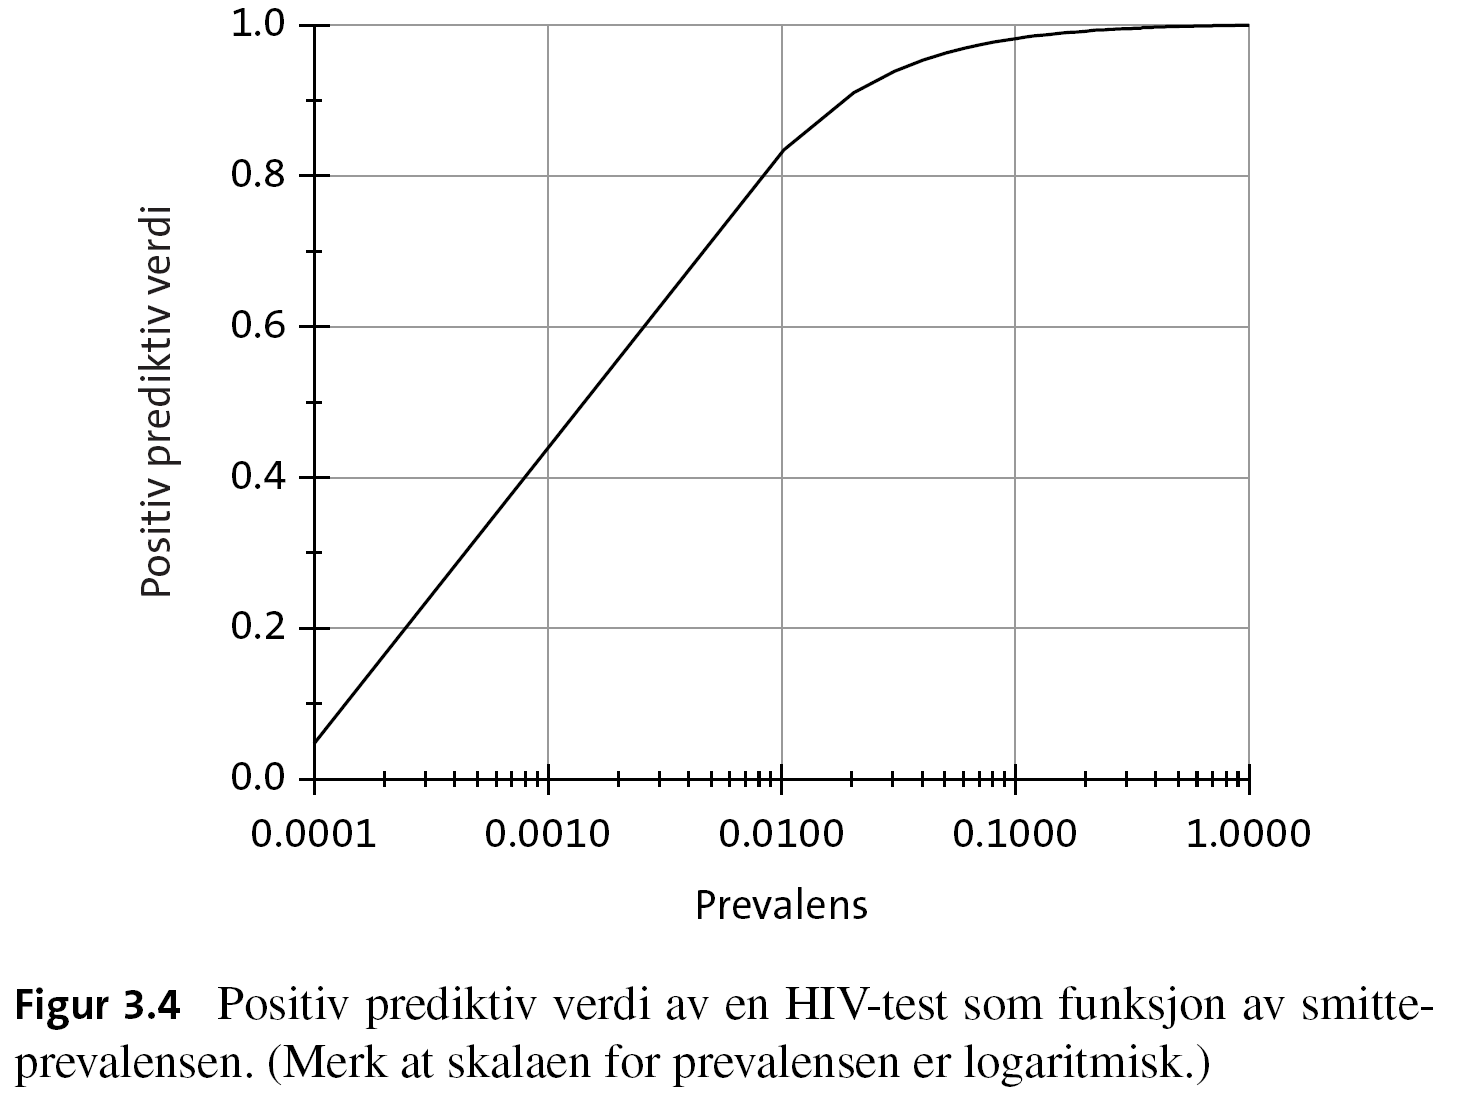
\includegraphics[height=0.70\textheight]{Figur3-4.png}
				%\caption{}
			\end{center}
		\end{figure}
	\end{block}
}

\frame{
	\frametitle{}
	\begin{block}{The importance of the prevalence}
		\begin{itemize}
			\item The \hl{risk of false positives depends strongly on the
				prevalence} -- it is greatest for rare diseases and smaller for
			more common diseases
			\item False positives are \hl{a big problem in mass screening} for
			disease. It could be that the majority of the positives are
			false positives
			
		\end{itemize}
	\end{block}
}




\section{Summary}

\frame{ 
\frametitle{Summary}
  \begin{block}{Key words}
    \begin{itemize}
    \item Sensitivity, specificity
    \item Positive predictive value, negative predictive value
    \end{itemize}
  \end{block}
}


\end{document}

